\chapter{Test Results and Simulations}
\label{ch:results}

In this chapter, we consider the problem of optimizing four standard functions in section \ref{sec:std-test-functions}, an ensemble of 200 GP sample functions in section \ref{sec:ensemble}, hyperparameter tuning of convolution network for classification in section \ref{sec:cnn-model}, and hyperparameter tuning for robotic arm in section \ref{sec:robotic}. Results are compared between algorithms \textit{Safeopt}, \textit{DistributedSafeOpt} and \textit{OverlappedDistributedSafeOpt} in terms of cumulative unsafe evaluations and achieved maxima. For all test runs and simulations we are initializing all three algorithms with same safe seed and kernel function.  

\section{Standard Test Functions}\label{sec:std-test-functions}
We are running our algorithm on four standard optimization functions, namely Bird function, Langermanns' function, Lavy05 function, and Michalewicz's function. These functions were chosen because they resemble what an irregular environment may seem like in real life. The steep slope of the Langermann function, for example, resembles an extremely deep oceanic trench, whereas the Bird function resembles a fluid diffusing away from an extraordinarily strong source. The performance is compared in terms of achievable maximum and cumulative unsafe evaluations. 
The performance is compared with \texttt{SafeOpt} algorithm as baseline. Details are discussed in following subsections.

\subsection{Bird Function}
Bird function is a 2-dimensional unimodal function, defined as
$$ f(x_1, x_2) = \sin(x_2) \exp (1-\cos(x_1))^2 + \cos(x_1)\exp(1-\sin(x_2))^2 + (x_1 - x_2)^2. $$
The function is usually optimized in search space $ [ (-2\pi, 2\pi), (-2\pi, 2\pi) ] $, and global minima is $f^*=-106.764537$ found at $(x_1, x_2)=(4.70104, 3.15294)$ and $(x_1, x_2)=(-1.58214, -3.13024)$.

Figure \ref{fig:bird-function-plot} shows the view of the function.

\begin{figure}[H]
	\centering
	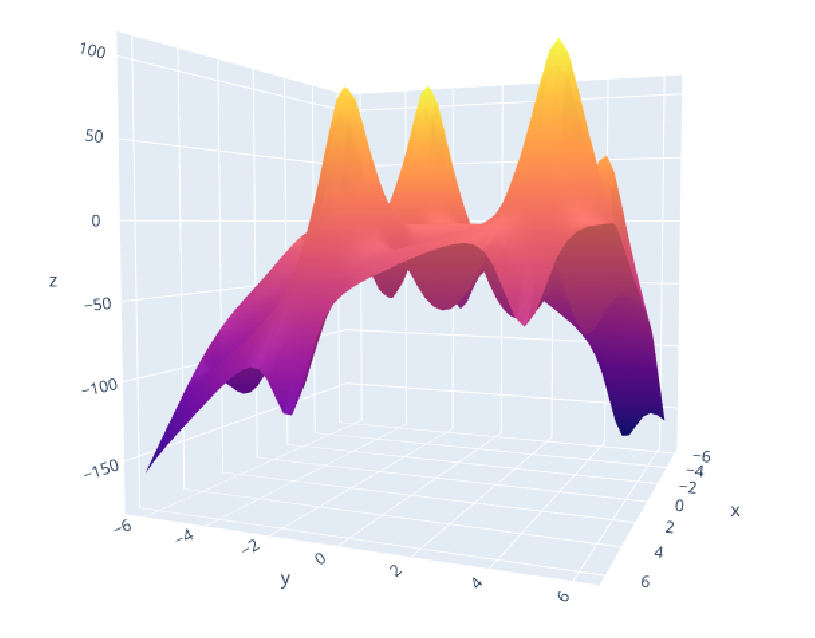
\includegraphics[scale=0.4]{figures/bird-function-plot.png}
	\caption{Bird function plot.}
	\label{fig:bird-function-plot}
\end{figure}

Figure \ref{fig:bird-result} shows a sample run on Bird function. Noise variance is $0.005^2$, RBF kernel (variance=1.0, lengthscale=1.0) as prior and safe seed $S_0=\{ (0,0) \}$ for safe threshold -35.0. From the results graph we can confirm that distributed version algorithms are also reaching same optima as SafeOpt without incurring not much more unsafe evaluations.
\begin{figure}[H]
	\centering
	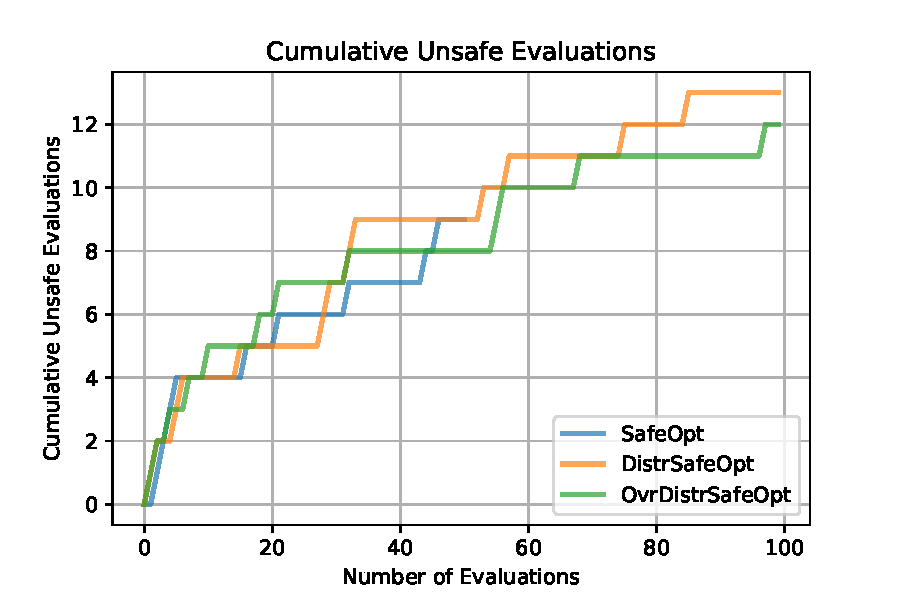
\includegraphics[width=0.65\textwidth]{figures/results/bird-cum-unsafe.pdf}
	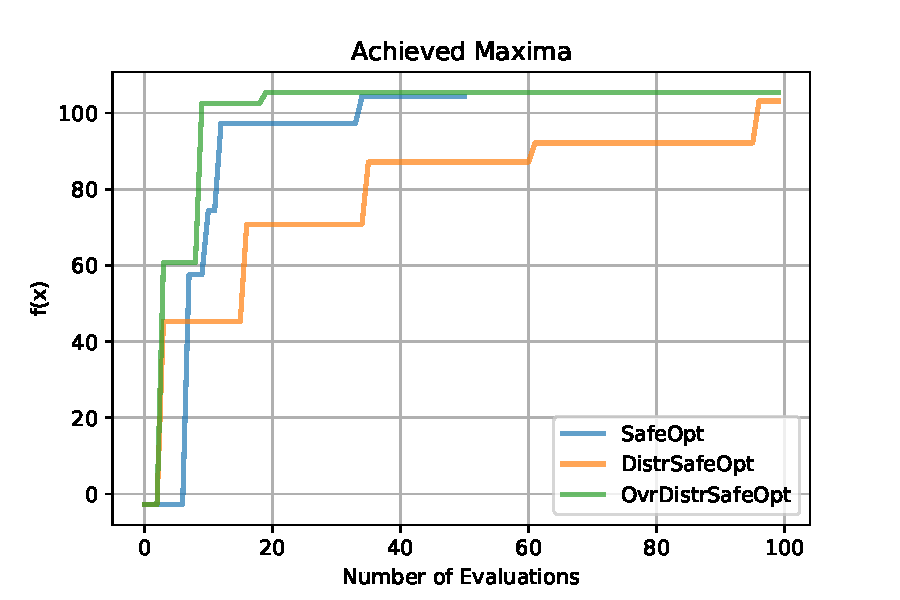
\includegraphics[width=0.65\textwidth]{figures/results/bird-maxima.pdf}
	\caption{Bird function results.}
	\label{fig:bird-result}
\end{figure}

\subsection{Langermanns' Function}
The Langermann function is a 2-dimensional test function with multiple minima. Unevenly distributed local minimas make optimization hard.
The function is defined as $$ f(x_1,x_2) = \sum_{i=1}^{m}c_i \exp(-(x_1-a_i)^2 / \pi - (x_2 - b_i)^2 / \pi) \cos(\pi (x_1-a_i)^2 + \pi (x_2 - b_i)^2) $$
We are considering the case where $m=5$ and $a=[3, 5, 2, 1, 7],$ $b = [5, 2, 1, 4, 9],$ and $c = [1, 2, 5, 2, 3]$. Search space is $[(3, 5), (3, 5)]$.

Figure \ref{fig:langermann-function-plot} shows the view of the function.
\begin{figure}[H]
	\centering
	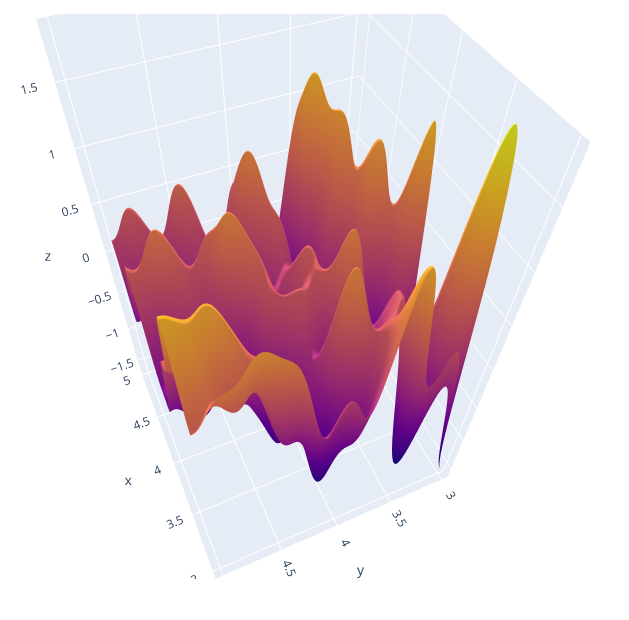
\includegraphics[scale=0.4]{figures/langermann-function-plot.png}
	\caption{Langermann function plot.}
	\label{fig:langermann-function-plot}
\end{figure}

Figure \ref{fig:langermann-result} shows a sample run on Langermann's function. Noise variance is $0.05^2$, Matern32 kernel (variance=0.5) as prior and safe seed $S_0=\{ (4.3,4.3)\}$ for safe threshold -0.5. From the results graph we can confirm that distributed version algorithms are also reaching same optima as SafeOpt without incurring not much more unsafe evaluations.
%\begin{figure}[h!]
%	\centering
%	\hspace*{-10em}
%	\begin{subfigure}{0.48\textwidth}
%		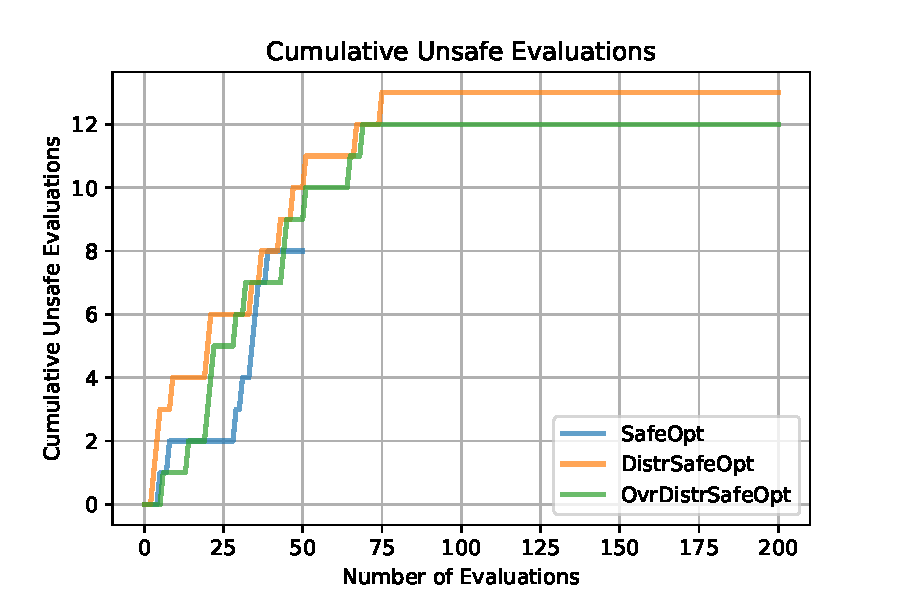
\includegraphics[scale=0.75]{figures/results/langermann-cum-unsafe.pdf}
%		\caption{}
%		\label{fig:langermann-cum-unsafe}
%	\end{subfigure}
%	\hspace*{7em}
%	\begin{subfigure}{0.48\textwidth}
%		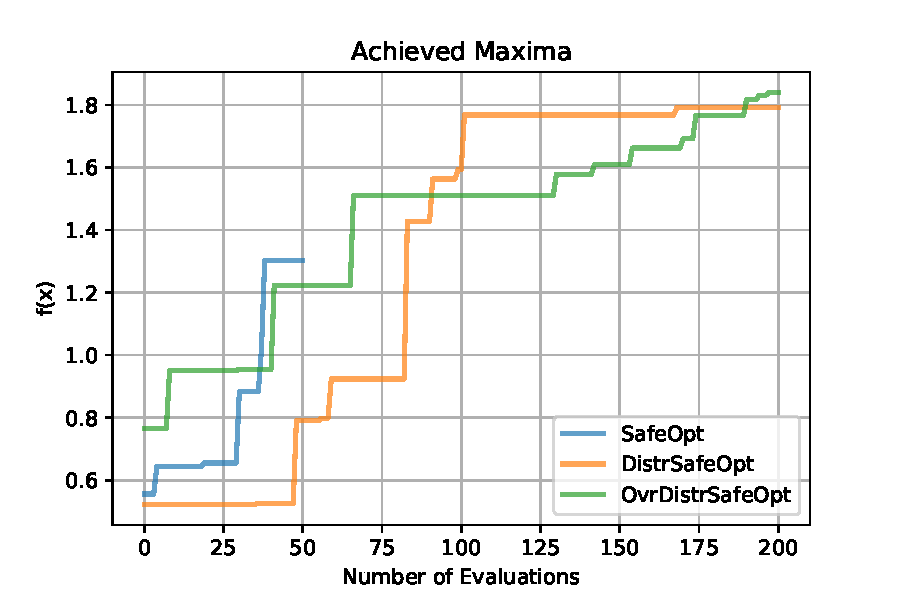
\includegraphics[scale=0.75]{figures/results/langermann-maxima.pdf}
%		\caption{}
%		\label{fig:langermann-maxima}
%	\end{subfigure}
%	\caption{Langermann's function results}
%	\label{fig:langermann-result}
%\end{figure}
\begin{figure}[H]
	\centering
	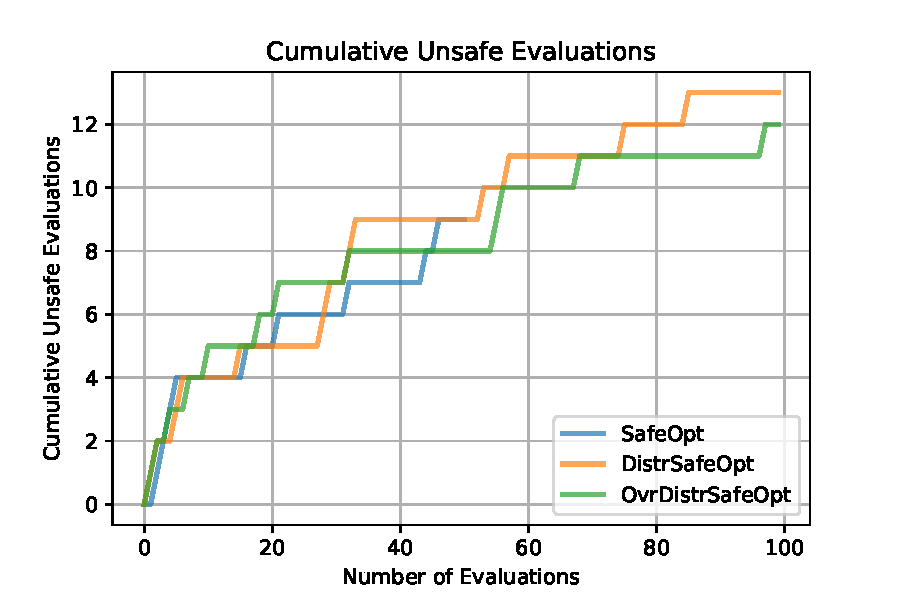
\includegraphics[width=0.65\textwidth]{figures/results/bird-cum-unsafe.pdf}
	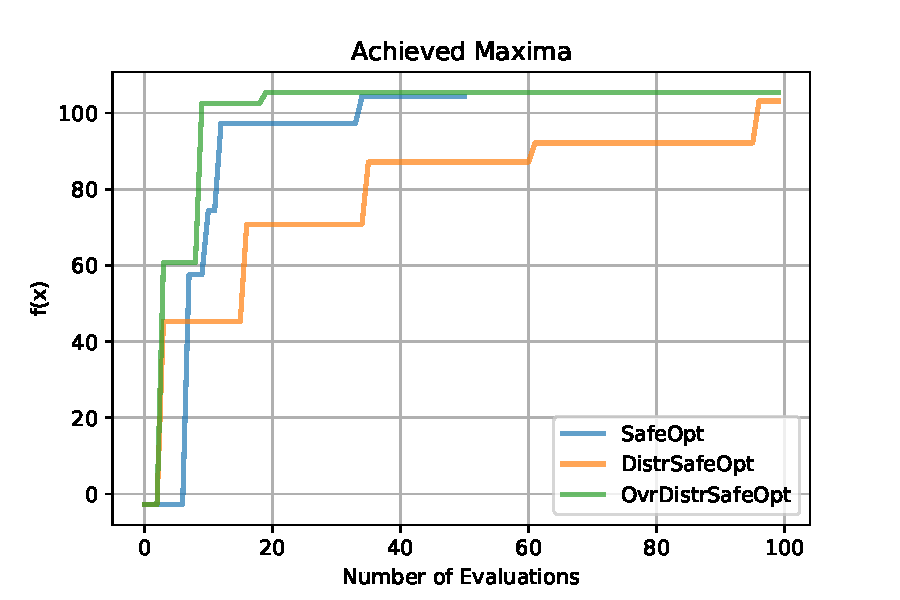
\includegraphics[width=0.65\textwidth]{figures/results/bird-maxima.pdf}
	\caption{Langermanns' function results}
	\label{fig:langermann-result}
\end{figure}

\subsection{Levy05 Function}
This is a multimodal optimization problem. Defined as
$$ f(x_1,x_2) = \sum_{i=1}^{5} i \cos[(i-1)x_1 + i] \times \sum_{j=1}^{5} j \cos[(j+1)x_2+j] + (x_1+1.42513)^2 + (x_2+0.80032)^2 $$
Search space is $[(-2, 2), (-2, 2)]$. And global minima is $f^*=176.1375$ at $(x_1, x_2)=(-1.3068, -1.4248)$. 

Figure \ref{fig:levy05-function-plot} shows the view of the function.
\begin{figure}[H]
	\centering
	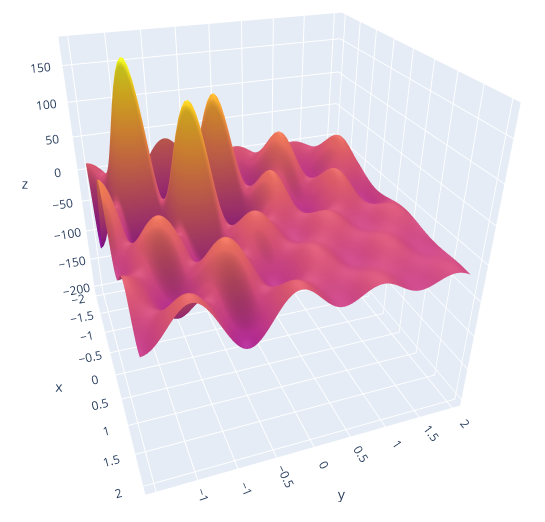
\includegraphics[scale=0.5]{figures/levy05-function-plot.png}
	\caption{Levy05 function plot.}
	\label{fig:levy05-function-plot}
\end{figure}

Figure \ref{fig:levy05-result} shows a sample run on Levy05 function. Noise variance is $0.5^2$, RBF kernel (variance=1.0, lengthscale=$[0.5, 0.25]$) as prior and safe seed $S_0=\{ (-0.8, -1.0) \}$ for safe threshold -50.0. From the results graph we can confirm that distributed version algorithms are also reaching same optima as SafeOpt without incurring not much more unsafe evaluations.
\begin{figure}[H]
	\centering
	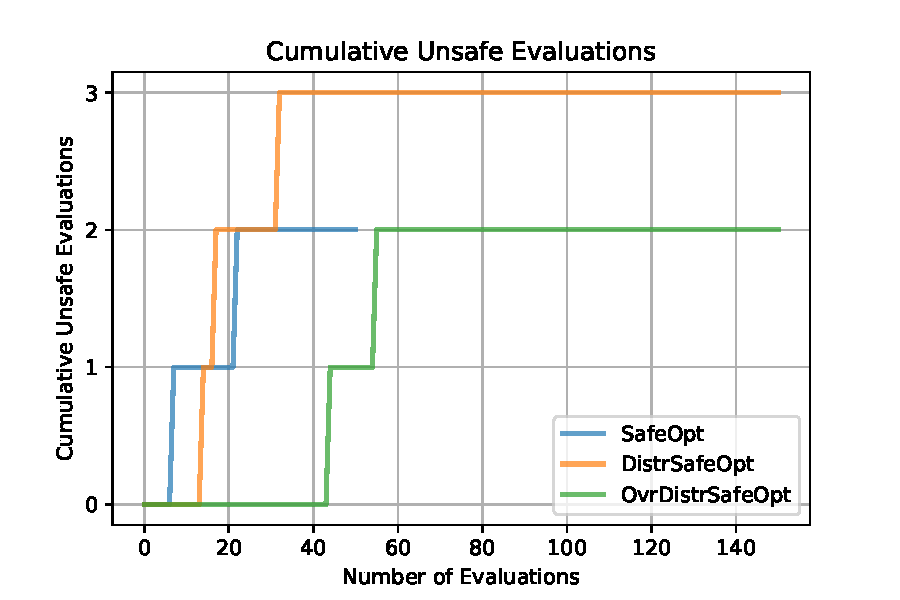
\includegraphics[width=0.65\textwidth]{figures/results/levy05-cum-unsafe.pdf}
	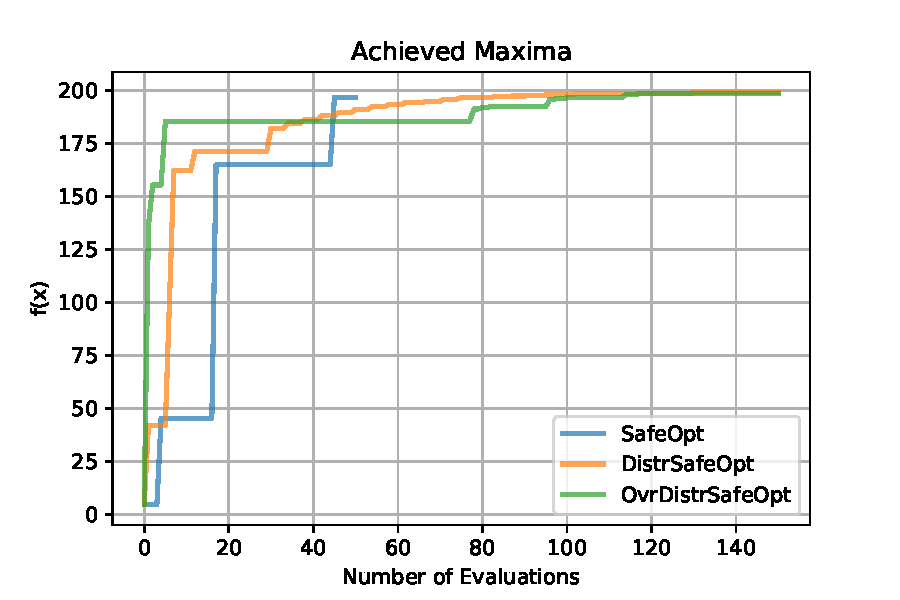
\includegraphics[width=0.65\textwidth]{figures/results/levy05-maxima.pdf}
	\caption{Levy05 function results}
	\label{fig:levy05-result}
\end{figure}

\subsection{Michalewicz's function}
The Michalewicz function is a $n$ dimensional test function. There are total $n!$ local optima available for this function.
The $m$ parameter determines how steep the valleys or edges are. The larger the $m$, the more difficult the search. The function acts like a needle in a haystack for extremely big $m$, and the function values for places beyond the narrow peaks provide very little information about the position of the global optimum.
Function has the following definition
$$ f(x) = -\sum_{i=1}^{n}\sin(x_i) \left[ \sin(\frac{ix_i^2}{\pi}) \right]^{2m}  $$
In our test we set $m=5$ and test area is restricted to hyphercube $0 \leq x_i \leq \pi,\ i = 1, \dots, n$. $f(x)=-4.687$ for $n=5$ has been used as approximate global minimum value. Respective optimal solutions are not given.

Figure \ref{fig:michalewicz-result} shows a sample run on Michalewicz function. Noise variance is $0.005^2$, RBF kernel (variance=1.0, lengthscale=0.5) as prior and safe seed $S_0=\{ (2, 3, 1, 2, 3) \}$ for safe threshold 0.8. From the results graph we can confirm that distributed version algorithms are also reaching same optima as SafeOpt without incurring not much more unsafe evaluations.
\begin{figure}[H]
	\centering
	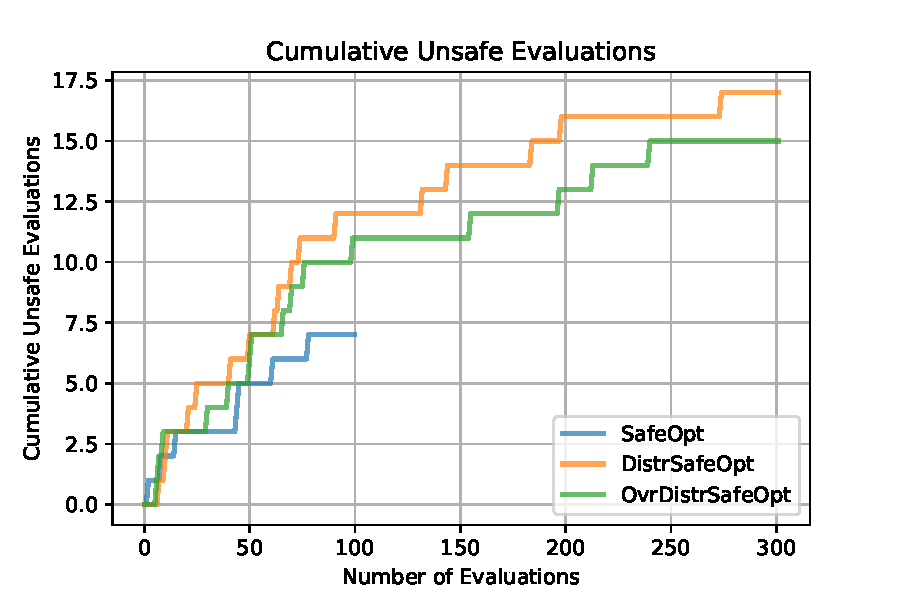
\includegraphics[width=0.65\textwidth]{figures/results/michalewicz-cum-unsafe.pdf}
	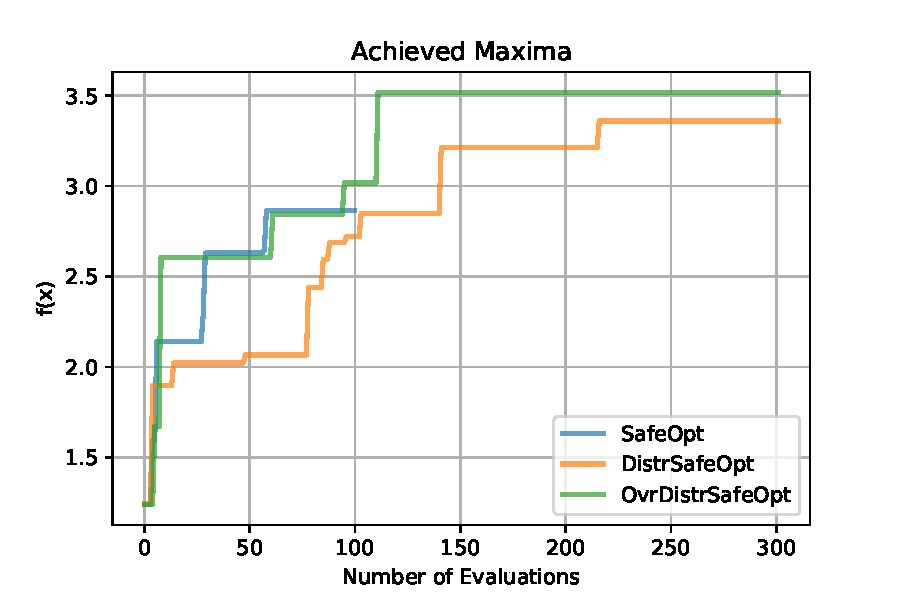
\includegraphics[width=0.65\textwidth]{figures/results/michalewicz-maxima.pdf}
	\caption{Michalewicz function results}
	\label{fig:michalewicz-result}
\end{figure}


\section{Ensemble of GP sample functions}\label{sec:ensemble}
Performance of all three algorithms is evaluated on an ensemble of 200 functions sampled from a GP prior and making 100 evaluations of each function. We have taken RBF kernel with parameters lenght scale $ls=1$ and variance $v=1$ as a prior for GP to generate required number of samples. Noise variance of functions set to $10^{-5}$.
Each function is defined on a domain $\mathcal{X}$: $([-10, 10], [-10, 10]) \subset \mathbb{R}^2$. Also each function $f(x)$ is scaled so that its maximum is 1 and minimum is 0. For scaling purpose maxima and minima of the functions are taken from the function evaluation over a $100\times100$ grid. For all functions we have taken point (0,0) as the safe seed for safe threshold 0.5. 

Figure \ref{fig:gp-sample-result} shows the results with solid line reprenting the mean value and shaded region for variance of the cumulative unsafe evaluations and achieved maxima taken over a total of 200 functions.
\begin{figure}[H]
	\centering
	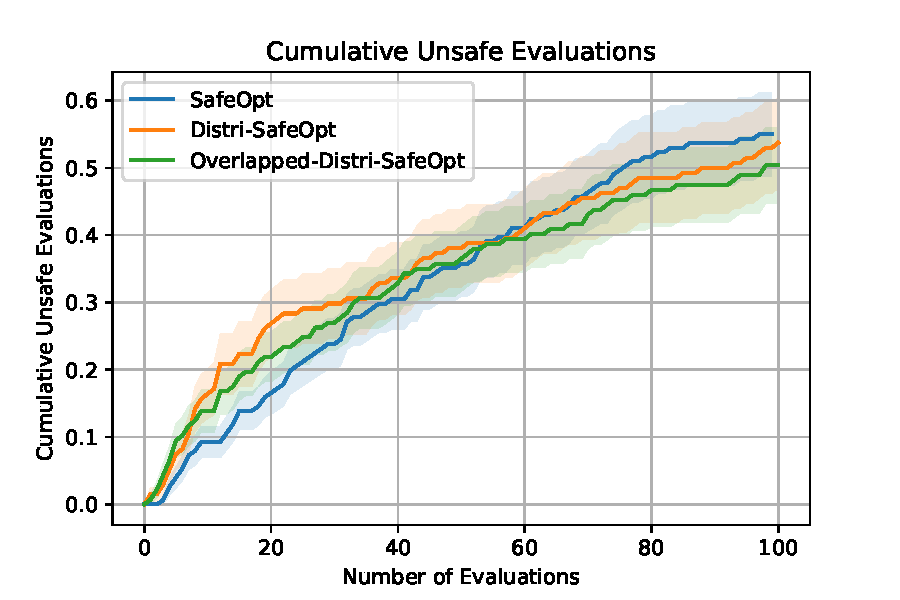
\includegraphics[width=0.65\textwidth]{figures/results/gp-sample-unsafe.pdf}
	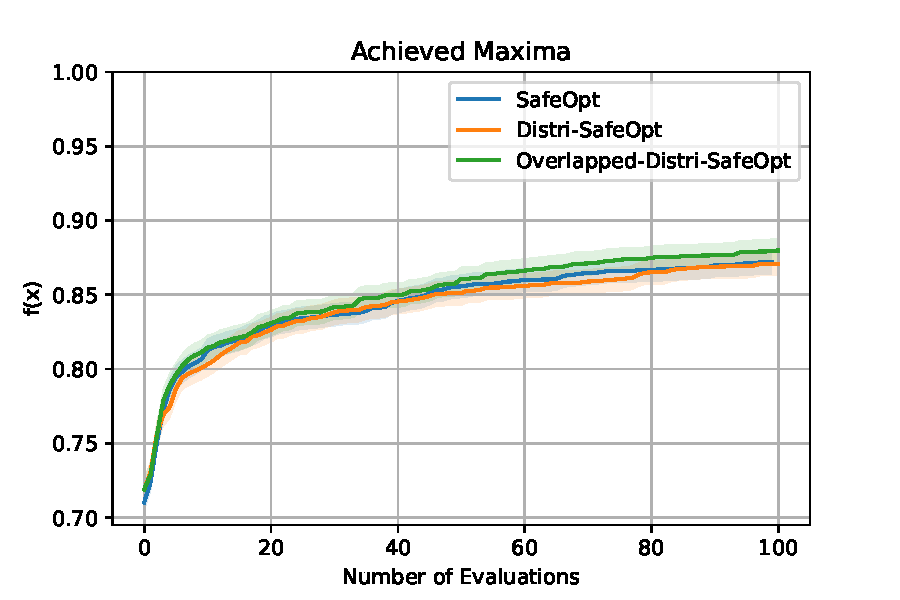
\includegraphics[width=0.65\textwidth]{figures/results/gp-sample-maxima.pdf}
	\caption{Ensemble of functions results}
	\label{fig:gp-sample-result}
\end{figure}


\section{CNN model hyperparameter tuning}\label{sec:cnn-model}
\textbf{Image Classification on CIFAR-10}: We experiment with tuning hyperparameters of a 5 layer convolutional neural network on an image classification task on the CIFAR-10 dataset \cite{cifar10}. This dataset contains 60000 $32\times32$ colour pictures divided into ten classes, each with 6000 images. There are 50000 images for training and 10000 images for testing.
\begin{figure}[H]
	\centering
	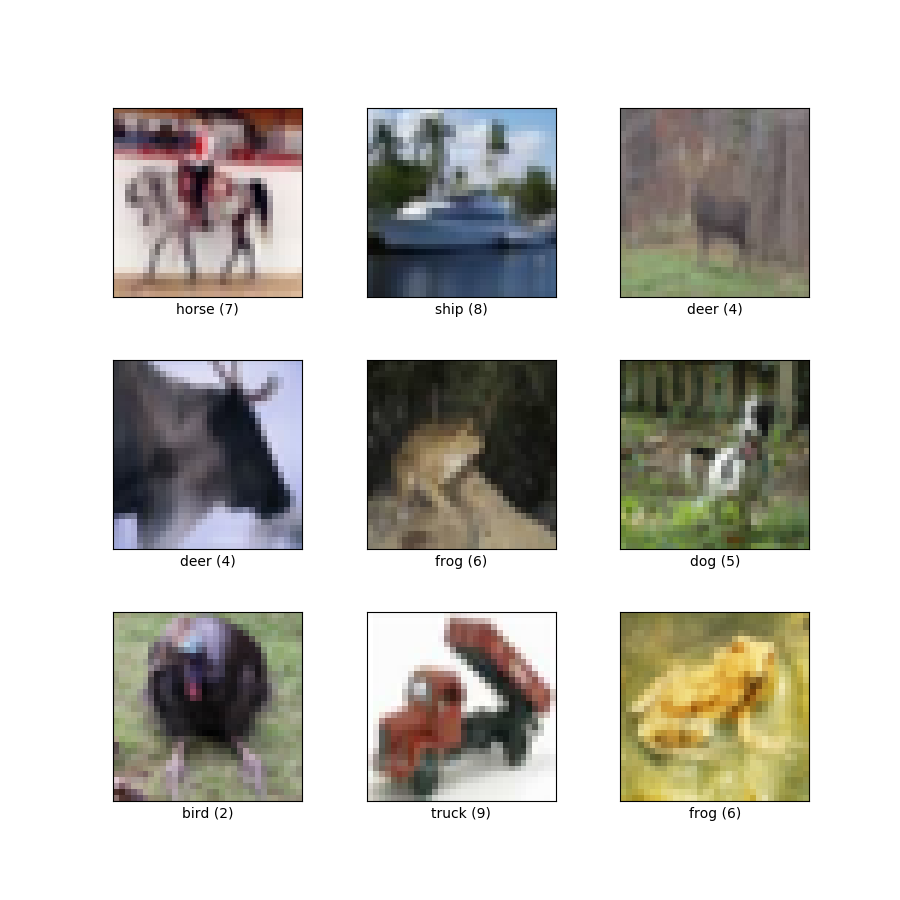
\includegraphics[scale=0.3]{figures/cifar10.png}
	\caption{A batch of images from CIFAR-10 dataset}
	\label{fig:cifar-10-dataset}
\end{figure}

We tune the learning rate $(10^{-5}, 10^{-1})$ and momentum $(0.05, 0.95)$ for Stochastic Gradient Descent (SGD) optimizer. The weights update equation for SGD is
$$ v_t = \gamma v_{t-1} + \eta \bigtriangledown w_t $$
$$ w_{t+1} = w_t - v_t $$
In the above equation, $w$ for weights, $\bigtriangledown w_t$ is the gradient of weights, $\eta$ is the learning rate, $\gamma$ is the momntum term, $v$ stands for velocity, and it accelerates gradients in the direction of convergence.

Here, each function evaluation trains the model on 50K images for 20 epochs and computes the test accuracy on a test set of 10K images.\\
Figure \ref{fig:cnn-result} shows the results. From the results graph we can confirm that distributed version algorithms are also reaching same optima as SafeOpt without incurring not much more unsafe evaluations.
\begin{figure}[H]
	\centering
	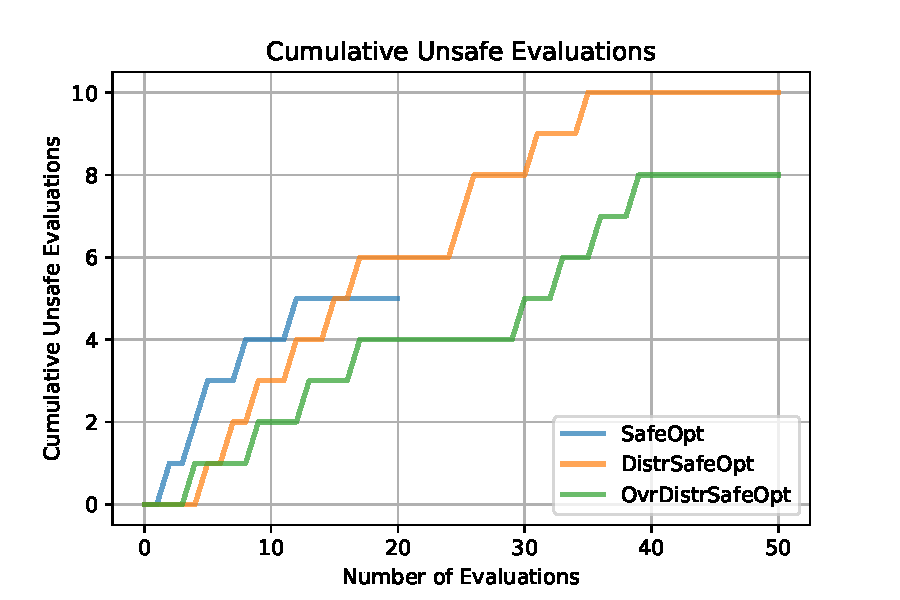
\includegraphics[width=0.65\textwidth]{figures/results/cnn-cum-unsafe.pdf}
	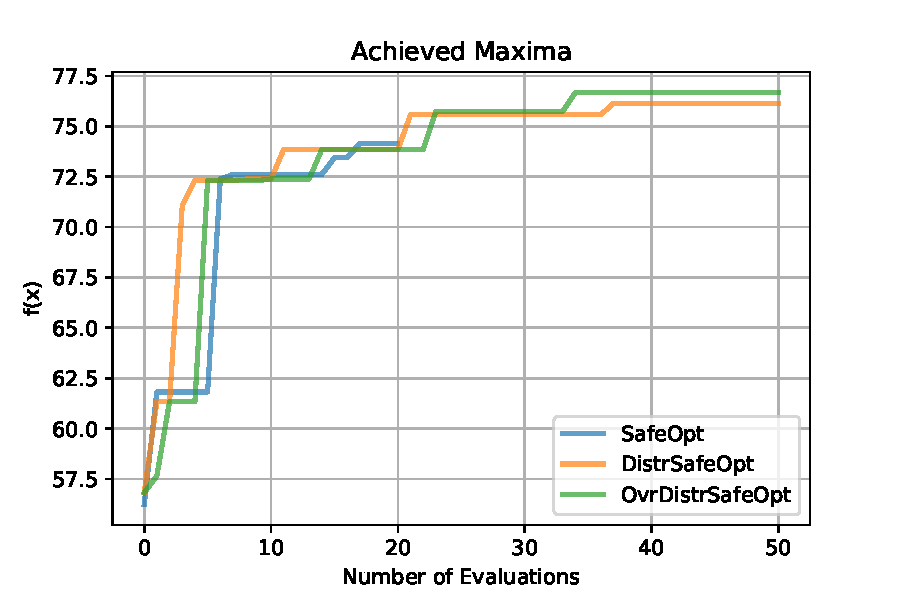
\includegraphics[width=0.65\textwidth]{figures/results/cnn-maxima.pdf}
	\caption{CNN model tuning results}
	\label{fig:cnn-result}
\end{figure}


\section{Hyperparameter tuning for Robotic Arm}
\label{sec:robotic}
In this section, we discuss a practical application of the algorithms mentioned in chapter \ref{ch:distbo}. The application setup consists of simulations done on the MuJoCo physics engine \cite{mujoco}. MuJoCo stands for Multi-Joint dynamics with Contact, is a physics engine designed for control tasks and joint dynamics. We use Linear Quadratic Regulator (LQR) to describe the robotic arm simulation system dynamics. The experiment consists of a robotic arm safely reaching a destination location $x_{des} \in \mathbb{R}^3$. The experiment is performed upon Franka Emika Panda's seven degrees of freedom (DOF) robot arm, shown in figure \ref{fig:panda-robot}.
%\footnote{URDFs and meshes are taken from \url{https://github.com/StanfordASL/PandaRobot.jl}}

We note that the objective function is an actual Black Box function as we only have access to function values when we interact with the system. We want the arm to reach the destination as quickly as possible, subject to underline safety constraints. The detailed discussion of objective and constraint functions is in the section \ref{subsec:exp-setup}. We compare the results with the SafeOpt algorithm and our algorithms DistributedSafeOpt and OverlappedDistributedSafeOpt.
\begin{figure}[H]
	\centering
	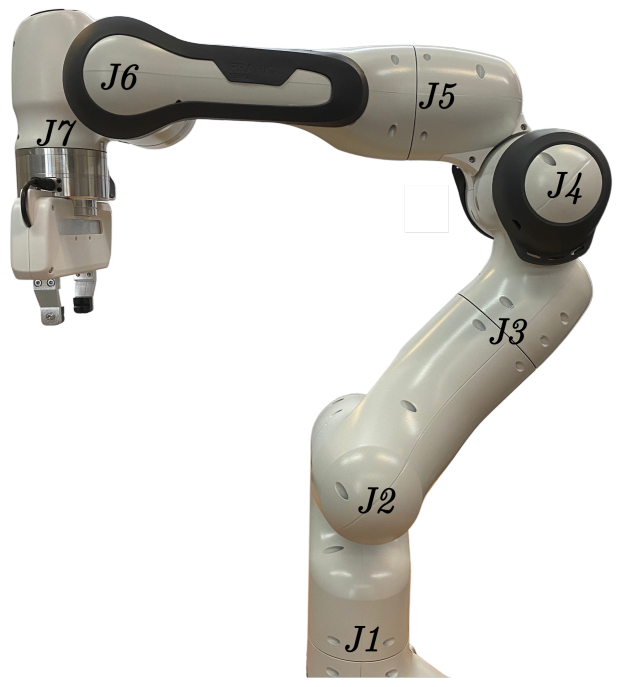
\includegraphics[scale=0.2]{figures/panda-robot.png}
	\caption{Franka Emika panda; seven degrees of freedom robot arm.}
	\label{fig:panda-robot}
\end{figure}

\subsection{Background}
\label{subsec:robot-prob-bg}
\hspace*{0.7cm}\textbf{Feedback Gain}: In a control system, when the complete or partial portion of the output is returned to the input side for utilization, then it is known as feedback gain.

\textbf{Linear Quadratic Regulator}: We consider a system that follows a discrete-time non-linear dynamic model
\begin{equation}
	\label{eq:dyn-model}
	x_{k+1} = f(x_k, u_k)
\end{equation}
with system states $x_k \in \mathbb{R}^{n_x}$ and control input $u_k \in \mathbb{R}^{n_u}$ at time instant $k$. We assume that (\ref{eq:dyn-model}) has an equilibrium at $x_k=0$ and $u_k=0$, which we want to keep the system at. We also assume that $x_k$ can be measured and, if not, an appropriate state estimator is used.

Consider a scenario, where a linear model
\begin{equation}
\label{eq:lin-system}
\tilde{x}_{k+1} = \boldsymbol{A}_n \tilde{x}_k + \boldsymbol{B}_n u_k
\end{equation}
is given as an approximation of the dynamics (\ref{eq:dyn-model}) about the equilibrium at zero. We refer to (\ref{eq:lin-system}) as the nominal model, while (\ref{eq:dyn-model}) are the true system dynamics, which are unknown.

A common way to measure the performance of a control system is through a quadratic cost function such as
\begin{equation}
\label{eq:lqr-cost-func}
J=\lim_{K \rightarrow \infty}\frac{1}{K}\mathbb{E}\left[\left(\sum_{k=0}^{K-1}x_k^{T}\boldsymbol{Q}x_k + u_k^{T}\boldsymbol{R}u_k\right)\right]
\end{equation}
with positive-definite weighting matrices $\boldsymbol{Q}$ and $\boldsymbol{R}$, and $\mathbb{E}[\cdot]$ the expected value. The cost (\ref{eq:lqr-cost-func}) captures a trade-off between control performance (keeping $x_k$ small) and control effort (keeping $u_k$ small).

A straightforward approach to compute the optimal controller minimizing (\ref{eq:lqr-cost-func}) for the nominal model (\ref{eq:lin-system}) will yield a locally optimal solution. This controller is given by the well-known Linear Quadratic Regulator (LQR) 
\begin{equation}
u_k = \boldsymbol{F}x_k
\end{equation}
whose static gain matrix $\boldsymbol{F}$ can readily be computed by solving the discrete-time infinite-horizon LQR problem for the nominal model $(\boldsymbol{A}_n, \boldsymbol{B}_n)$ and the weights $(\boldsymbol{Q}, \boldsymbol{R})$. For simplicity, we write
\begin{equation}
\label{eq:lqr}
\boldsymbol{F} = lqr(\boldsymbol{A}_n, \boldsymbol{B}_n, \boldsymbol{Q}, \boldsymbol{R})
\end{equation}

\textbf{Feedback Linearization}: It is a technique used to produce a different linear system that represents the original nonlinear system. Two steps are involved in Feedback Linearization: operations performed to change the coordinate system into a nonlinear one and the application of nonlinear feedback.

If (\ref{eq:lin-system}) can comprehend the exact dynamics of the system, then we can design the optimal controller for the system at hand. If not, we will have nonlinearities which need to be minimised. To solve the equation (\ref{eq:lqr}) we introduce the parametrization of the matrices $\boldsymbol{Q}$ and $\boldsymbol{R}$. We initialise $\boldsymbol{Q}(\theta) \sim q : \theta \in \mathbb{R}^d$ and $\boldsymbol{R}(\theta) \sim r : \theta \in \mathbb{R}^d$.
While varying $\theta$, we can obtain various controller gain $\boldsymbol{F}$. We observed these gains and made decisions accordingly. Thus, the cost matrix now depends on $\theta$ such that
\begin{equation}
J=J(\theta)
\end{equation}
The goal of the automatic LQR tuning is to vary the parameters $\theta$ such as to minimize the cost (\ref{eq:lqr-cost-func}).

\subsection{Experiment Setup}
\label{subsec:exp-setup}
This section discusses the setup for the simulation experiment on a Franka Emika Panda seven degree of freedom (DOF) robot arm. The experiment involves the control task of the robot arm to reach a fixed position $x_{des} \in \mathbb{R}$ as quickly as possible without violating safety constraints \cite{gosafeopt}.

To determine the impedance gain, we use an approximate system model and perform feedback linearization. For the resulting linear system, we design a linear-quadratic regulator (LQR) with quadratic costs parameterized by matrices $\boldsymbol{Q}$ and $\boldsymbol{R}$. Since the model is inaccurate, the feedback linearization will not cancel all nonlinearities the LQR will not be optimal. 

Thus, our goal is to tune the cost matrices Q and R to compensate for the nonlinearities. Formally we define the system model as
\begin{equation}\label{eq:modellqr}
u(x(t)) = \Lambda(q) \ddot{s} + \Gamma(q,\dot{q})\dot{s} + \eta(q),
\end{equation}
where $s$ represents the end-effector position, $q$ the joint angles, and $\Lambda(q)$,
$\Gamma(q,\dot{q})$, $\eta(q)$ are nonlinearities representing the mass, Coriolis, and gravity terms, respectively. The state we consider is $x(t)=[s^T(t), \dot{s}^T(t)]^T$.

We apply an impedance controller:
\begin{equation}
	u(x(t)) = -\boldsymbol{F}\begin{bmatrix}
		s\\
		\dot{s}
	\end{bmatrix} + \Gamma(q,\dot{q})\dot{s} + \eta(q),
\end{equation}
with $\boldsymbol{F}$ being the feedback gain. The torque $\tau$ applied to each of the joints can be calculated via $\tau = J^Tu(x(t))$, with $J$ the Jacobian.

For the simulation task, we determine the impedance $\boldsymbol{F}$ using an infinite horizon LQR parameterized via
\begin{equation*}
	\boldsymbol{Q} = \begin{bmatrix}
		\boldsymbol{Q}_r & 0\\
		0 & \kappa_d\boldsymbol{Q}_r
	\end{bmatrix}, \boldsymbol{Q}_r=10^{q_c}I_3,
\end{equation*}
\begin{equation*}
	 \boldsymbol{R}=10^{r-2}I_3,  \boldsymbol{A} = \begin{bmatrix}
	 	0 & I_3\\
	 	0 & 0
	 \end{bmatrix}, \boldsymbol{A}=\begin{bmatrix} 0\\I_3
	\end{bmatrix}.
\end{equation*}
The matrices $\boldsymbol{A}$, $\boldsymbol{B}$ are obtained assuming that we use a feedback linearization controller. However, because we instead use an impedance conntroller, there are nonlinearities and imprecisions in our model. The parameters $q_c$, $r$, $\kappa_d$ are tuning parameters we would like to optimize. Such an approach is in tune with \cite{LQR}.

Our model encourages the end-effector position of the robot to reach the destination as fast as possible while penalizing high end-effector velocities.
The constraint and stage rewards (i.e., rewards received at each time step) are:

\begin{center}
	$\begin{aligned}
	\bar{g}(x(t))=& \frac{\left\|s(t)-s_{\text {des }}\right\|_{2}-\left\|s(0)-s_{\text {des }}\right\|_{2}}{\left\|s(0)-s_{\text {des }}\right\|_{2}}-\alpha, \quad \alpha=0.08 \\
	\mathcal{R}(x(t))=&-\left\|s(t)-s_{\mathrm{des}}\right\|_{2}^{2} /\left\|s(0)-s_{\operatorname{des}}\right\|_{2}^{2} \\
	&-\frac{1}{25}\|\tanh \dot{s}(t)\|_{2}^{2}-\frac{1}{25}\|\tanh u(x(t))\|_{2}^{2}
	\end{aligned}$
\end{center}
 
The task at hand is a high dimensional one as we have six states representing the robot's joint positions and the two parameters $q_c$ and $r$. We restrict our parameter search space to a normalized domain $q_n \times r_n \in [1/3,1] \times [-1,1]$ with $q_c = 6q_n$ and $r = 3r_n$. The value for $\kappa_d$ is heuristically set to 0.1 \cite{gosafeopt}.

\subsection{Simulation Results and Comparison}
We evaluate our algorithms \textit{DistributedSafeOpt} and \textit{OverlappedDistributedSafeOpt} in a simulation environment based on the MuJoCo physics engine. And compare the results with \textit{SafeOpt}. 

The safe seed $S_0$ is initialized with three safe points $[\frac{4}{6},-1],[\frac{5}{6},0.9],[1,-\frac{2}{3}]$. We are using \textit{sde\_Matern32} kernel (Matern covariance functions with the Stochastic Differential Equation (SDE) functionality) with lenghtscale set to $\frac{0.7}{6}$.
We use two GPs to model the system. The first GP models the objective function with $-\infty$ as the safe threshold, and the other models the constraint function with 0 as the safe threshold.
We are running the \textit{SafeOpt} algorithm for 200 iterations. For \textit{DistributedSafeOpt} algorithm, we are dividing both search dimensions into two subspaces which gives us four possible hyperspaces in total. Same for \textit{OverlappedDistributedSafeOpt} algorithm also with 15\% of search space overlap. Both these algorithms are evaluated for 500 iterations.

All three algorithms evaluated zero unsafe points and distributed version algorithms achieved higher maxima. These results are shown in figure \ref{fig:robot-result}.

\begin{figure}[h!]
	\centering
	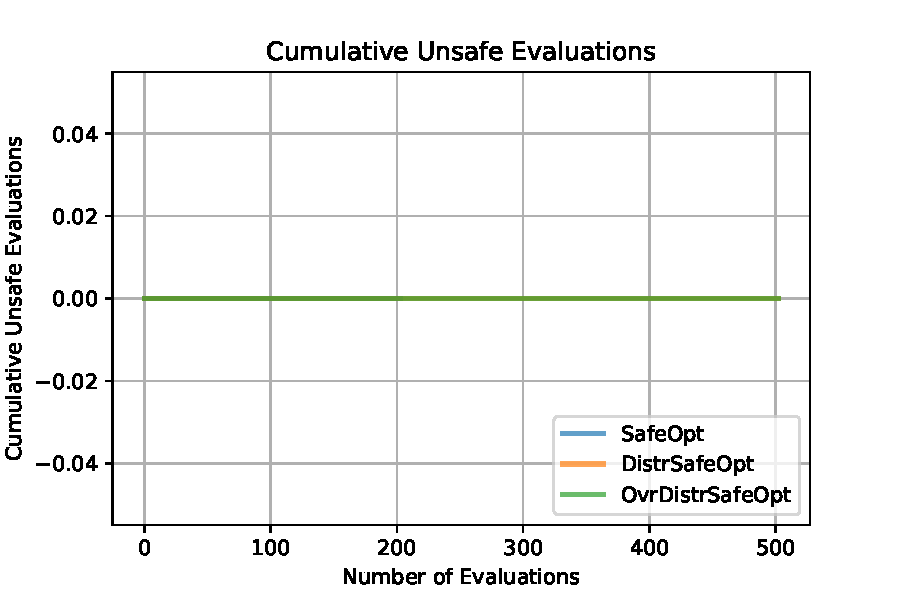
\includegraphics[width=0.65\textwidth]{figures/results/robot-cum-unsafe.pdf}
	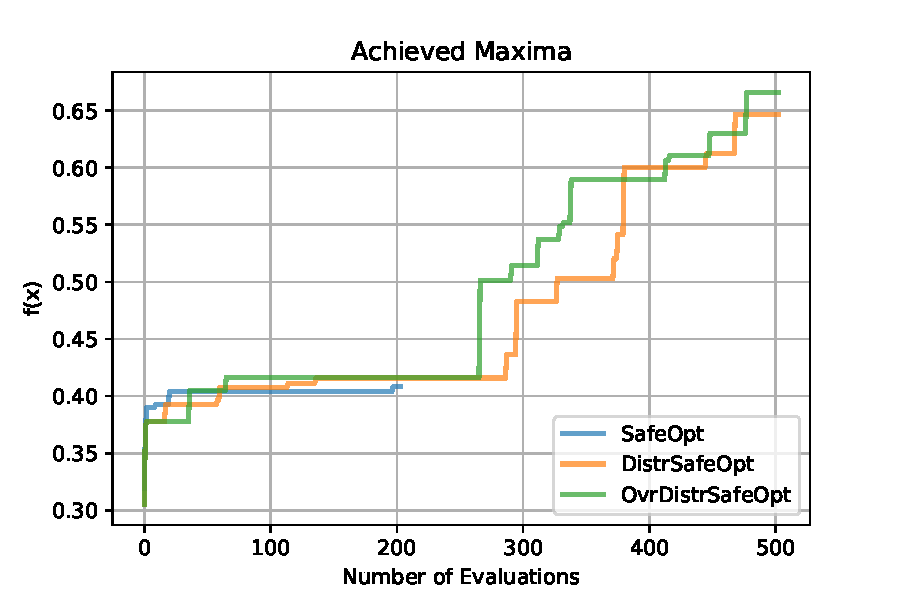
\includegraphics[width=0.65\textwidth]{figures/results/robot-maxima.pdf}
	\caption{Robotic arm simulation report}
	\label{fig:robot-result}
\end{figure}


Figure \ref{fig:safeset-result} shows the safe set belief and maxima by all three algorithms at the end of the optimization process. Since the distributed algorithms evaluated more points than a sequential algorithm, the safe set discovered by them is broader and resulted in reaching higher maxima.

\begin{figure}[h!]
	\centering
	\hspace*{-5.6em}
	\begin{subfigure}{0.32\textwidth}
		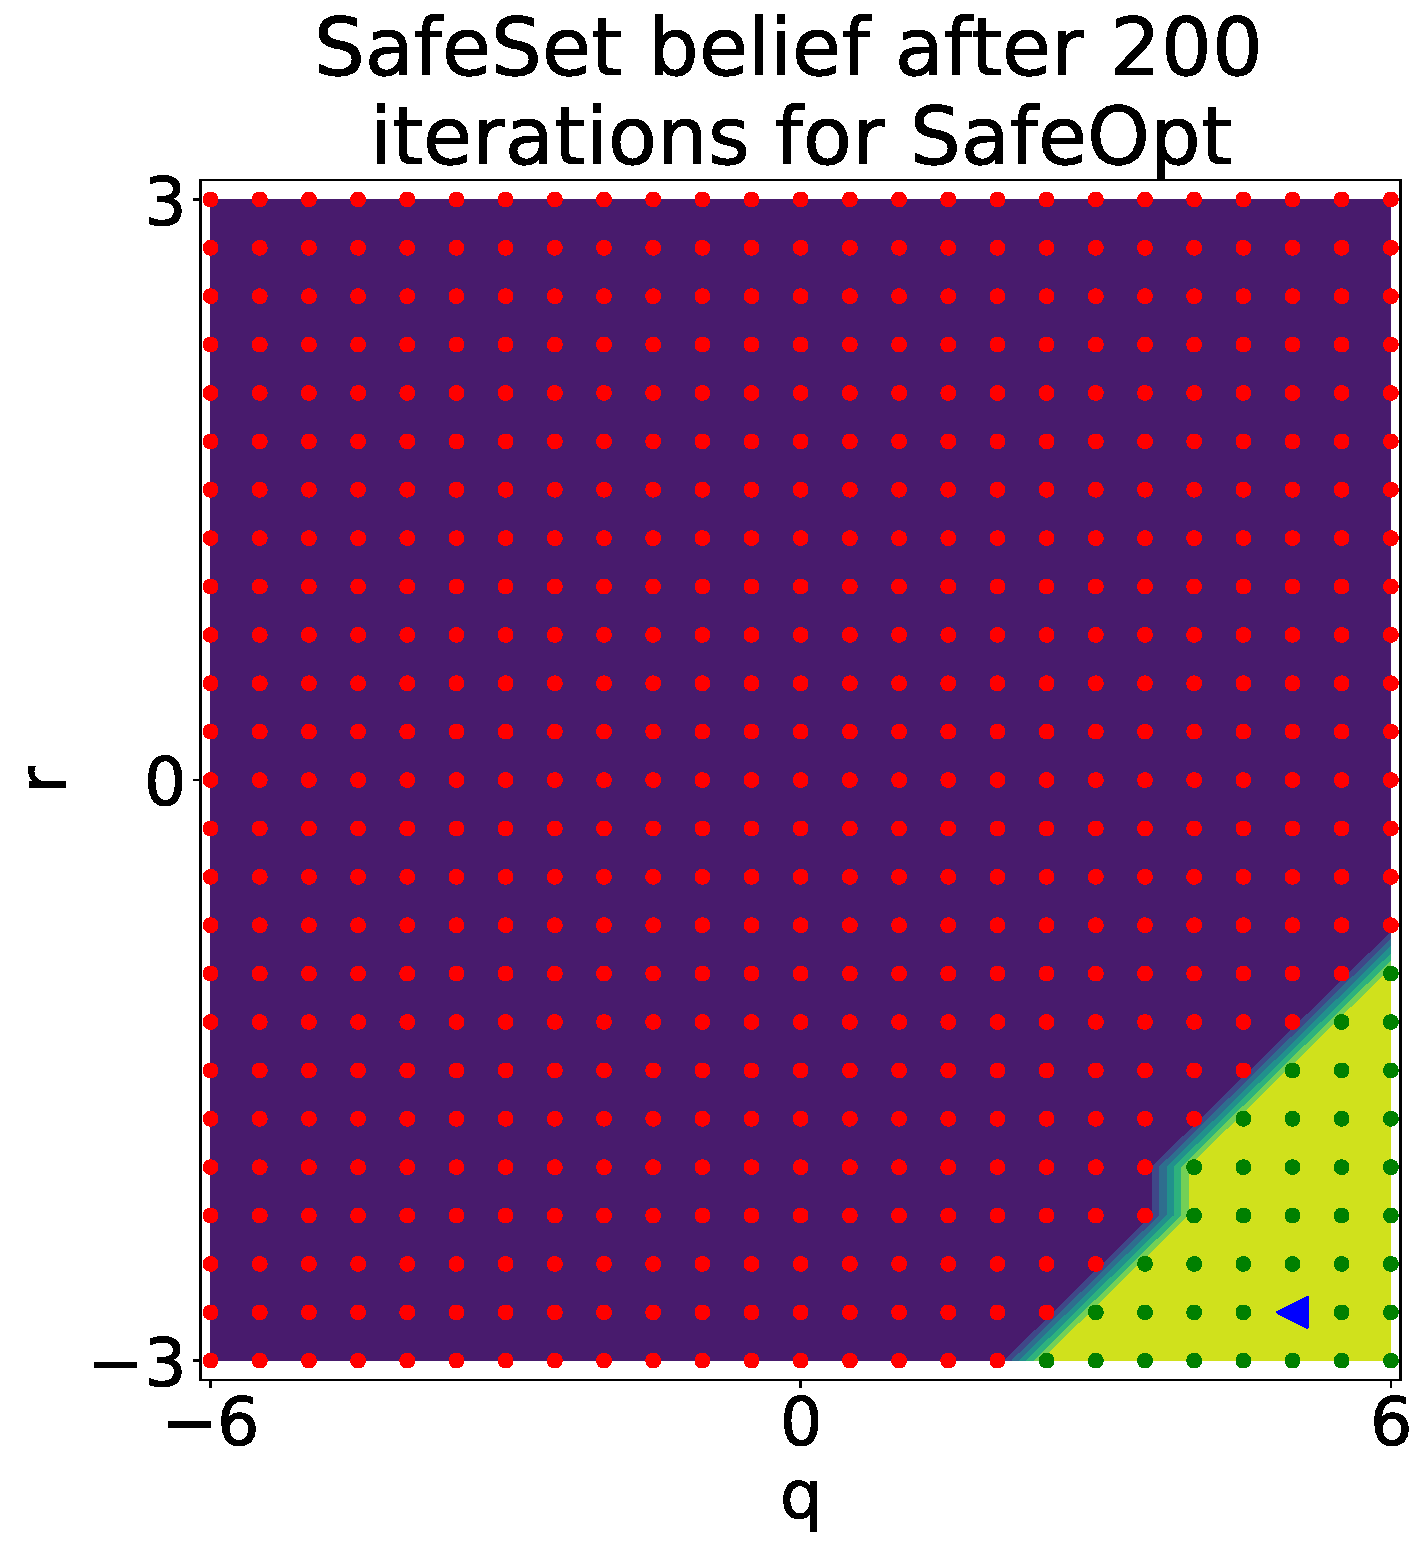
\includegraphics[scale=0.25]{figures/results/robot-sbo-safeset-200.pdf}
		\caption{}
		\label{fig:safeopt-safeset}
	\end{subfigure}
	\hspace*{2.2em}
	\begin{subfigure}{0.32\textwidth}
		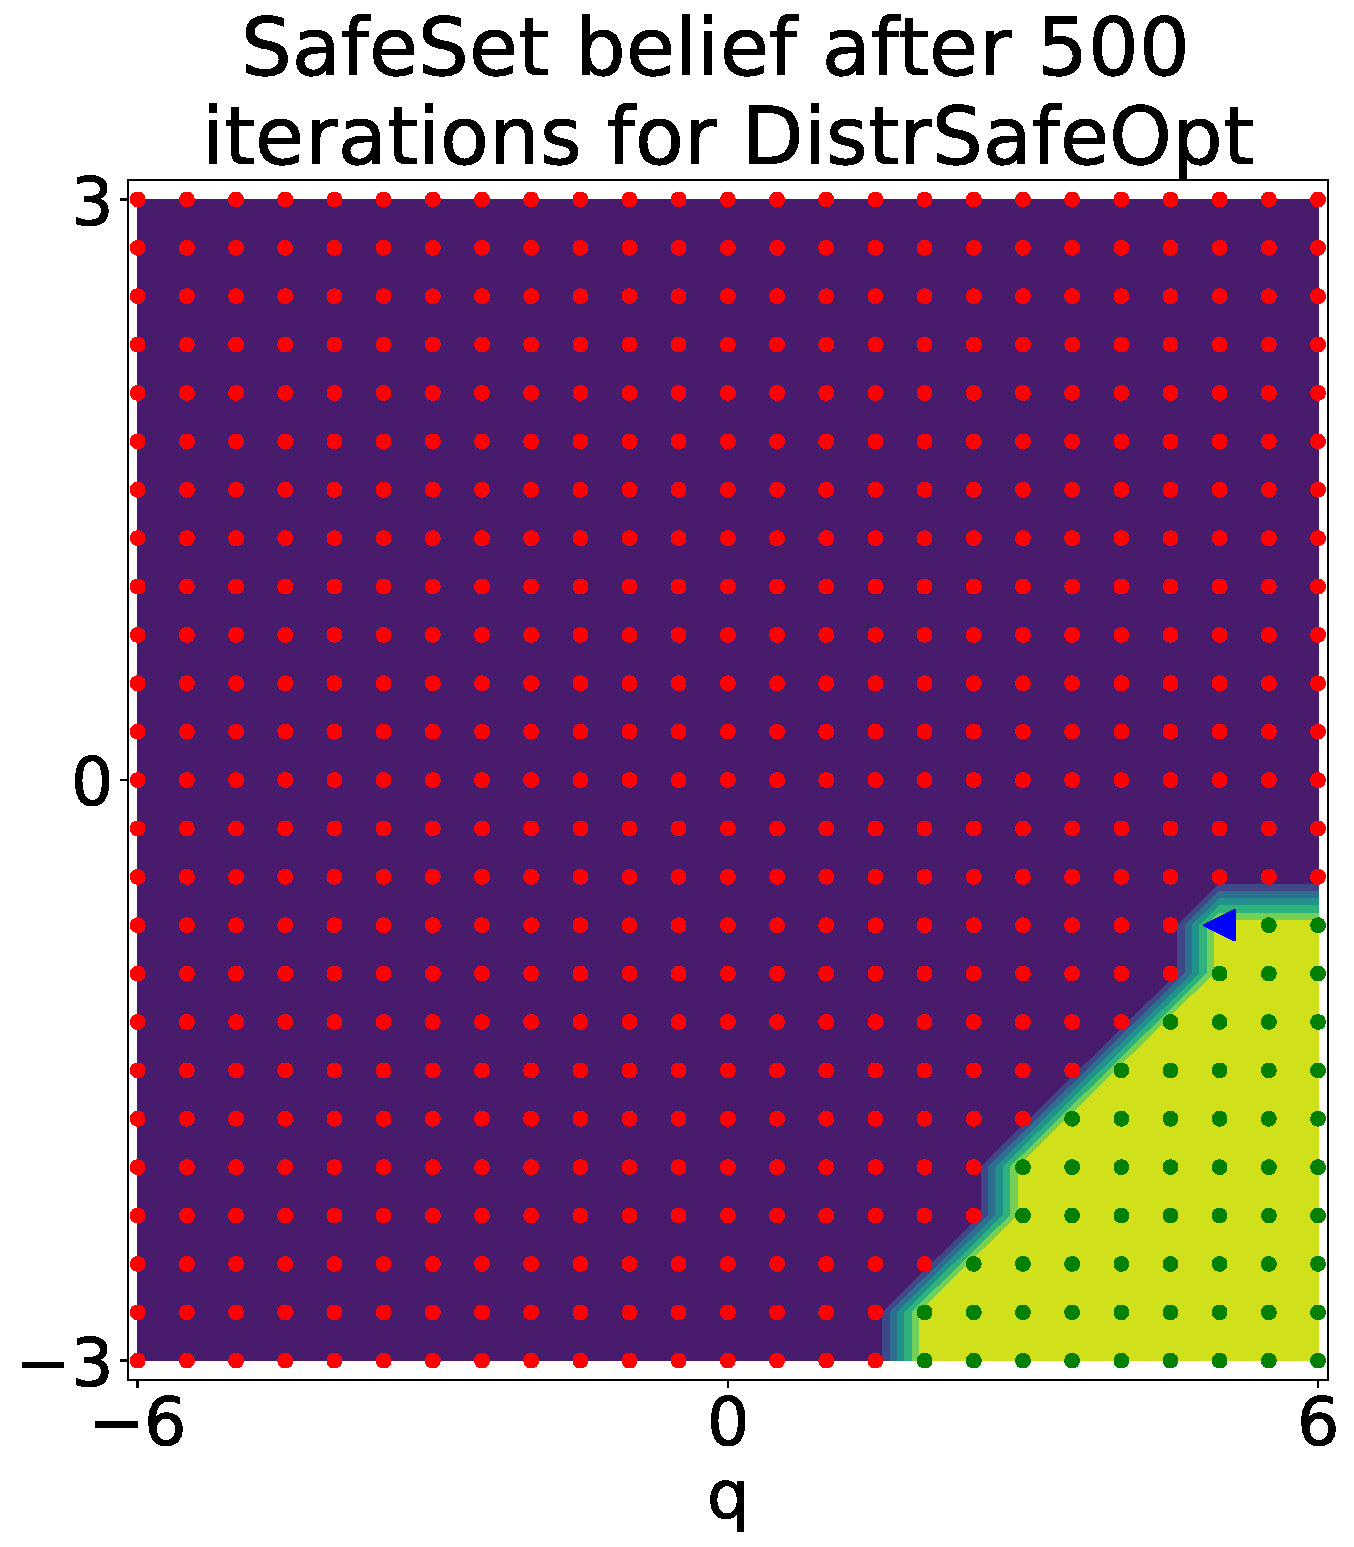
\includegraphics[scale=0.25]{figures/results/robot-dbo-safeset-500.pdf}
		\caption{}
		\label{fig:dbo-safeset}
	\end{subfigure}
	\hspace*{1.8em}
	\begin{subfigure}{0.32\textwidth}
		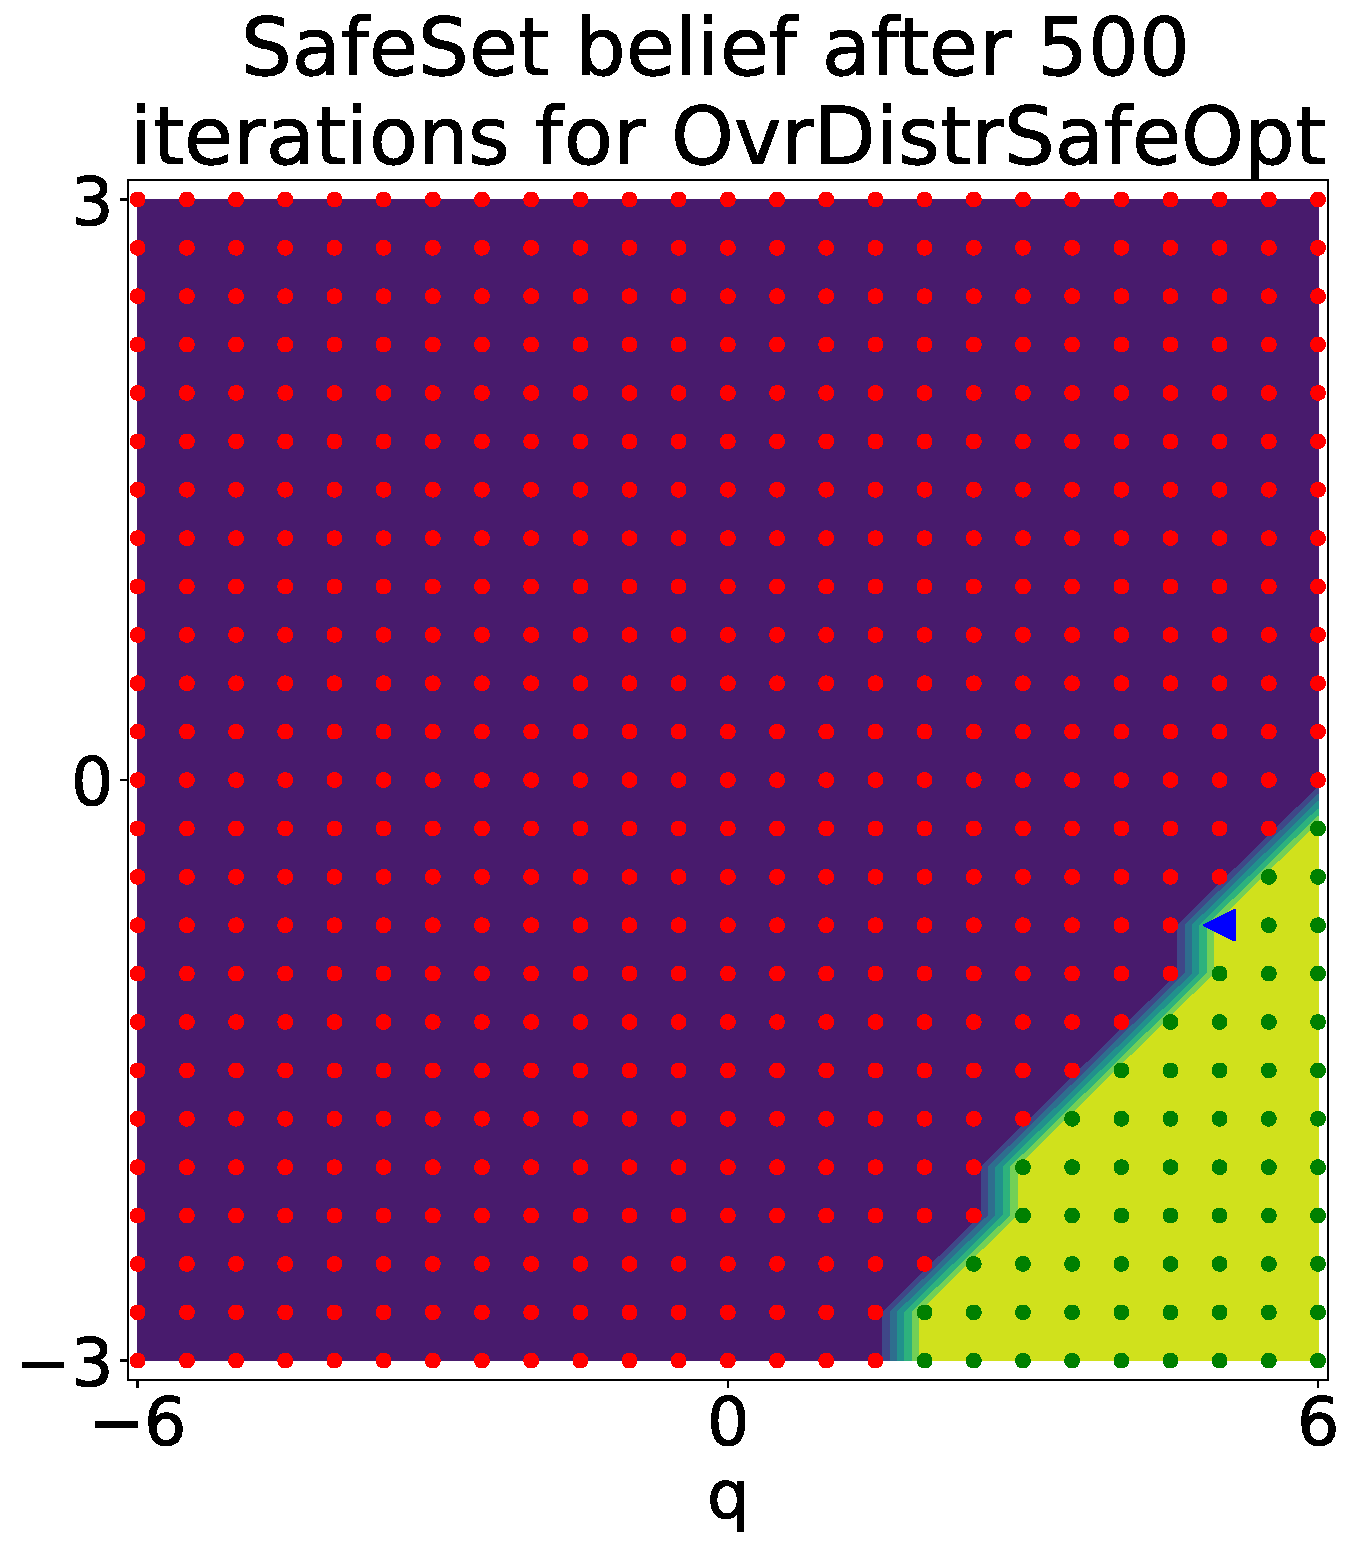
\includegraphics[scale=0.25]{figures/results/robot-ovr-safeset-500.pdf}
		\caption{}
		\label{fig:ovr-safeset}
	\end{subfigure}
	\caption{Safe Set belief}
	\label{fig:safeset-result}
\end{figure}